\documentclass[11pt,a4paper]{article}
\usepackage[utf8]{inputenc}
\usepackage[spanish,es-tabla]{babel}
\usepackage{amsmath}
\usepackage{amsfonts}
\usepackage{amssymb}
\usepackage{graphicx}

\usepackage{vmargin}

\setpapersize{A4}
\setmargins{2.5cm}              % margen izquierdo
{1.5cm}                         % margen superior
{16.5cm}                        % anchura del texto
{23.42cm}                       % altura del texto
{10pt}                          % altura de los encabezados
{1cm}                           % espacio entre el texto y los encabezados
{0pt}                           % altura del pie de página
{2cm}                           % espacio entre el texto y el pie de página

\title{ 
    Emisión de titulos universitarios
    en la Blockchain
}
\author{
    Saez, Lautaro Andres \\ \small{ LautaroAndresSaez@gmail.com } 
    \and 
    Riperto, Adriel Aaron \\ \small{ aaron.ariperto@gmail.com } 
}
\date{\today}

\begin{document}
    \maketitle

    \section{Introducción}

    \section{Estado del arte}

        Esta sección tiene como objetivo tratara el estado actual de la tematica a abordar.
        Debido a que blockchain se encuentra en constante crecimiento, no hay una gran cantidad 
        de trabajos implementados en el ambito sobre los titulos academicos. Pero se investigo 
        y encontraron dos propuestas sobre el tema. %Correguir implementaciones!

        \subsection{Blockchain federal Argentina (BFA)}


        Blockchain Federal Argentina es una plataforma multiservicios abierta y participativa pensada en integrar servicios y aplicaciones
        sobre blockchain. % Referencia https://bfa.ar/bfa/que-es-bfa
        
        BFA propone multiples casos de uso para blockchain, entre ellos se encuentra una propuesta donde el alumno pueda solicitar
        el titulo academico, la universidad valide la aprobacion de las materias y el ministerio de educacion certifique el titulo.

        Esto se propone lograrlo empleando “sellos de tiempo” donde es posible garantizar que los documentos involucrados 
        no puedan ser alterados. Estos generan digestos criptográficos (hash) de historias académicas o títulos que quedan 
        almacenados en la blockchain y a través de ellos se puede garantizar que los mismos no han recibido modificaciones 
        indebidas en todo el proceso. % Referencia https://bfa.ar/blockchain/casos-de-uso/titulos-academicos

        Las ventajas que presenta esta solucion son:
        
        \begin{itemize}
            \item Garantiza que no sea posible alterar la 
            información de las actas sin que esa modificación sea detectada y así aumenta la confianza en la autenticidad de los títulos emitidos. 
            \item Transparencia en el proceso de digitalización.
            \item Permite un contexto de confianza entre organismos y partes interesadas. 
            \item Auditable.
            \item Permite demostrar que no existen actos de negligencia (títulos truchos) en torno a la emisión de títulos.
            \item Se podría dar diferentes vigencias a certificado de títulos en trámite, o similares, certificadas en la blockchain.
        \end{itemize}

        Por otro lado se proponen posibles mejoras a esta implementción creando un portafolios digital, lo cual 
        permitiria modificar los permisos de acceso.

        \begin{figure}
            \centering
            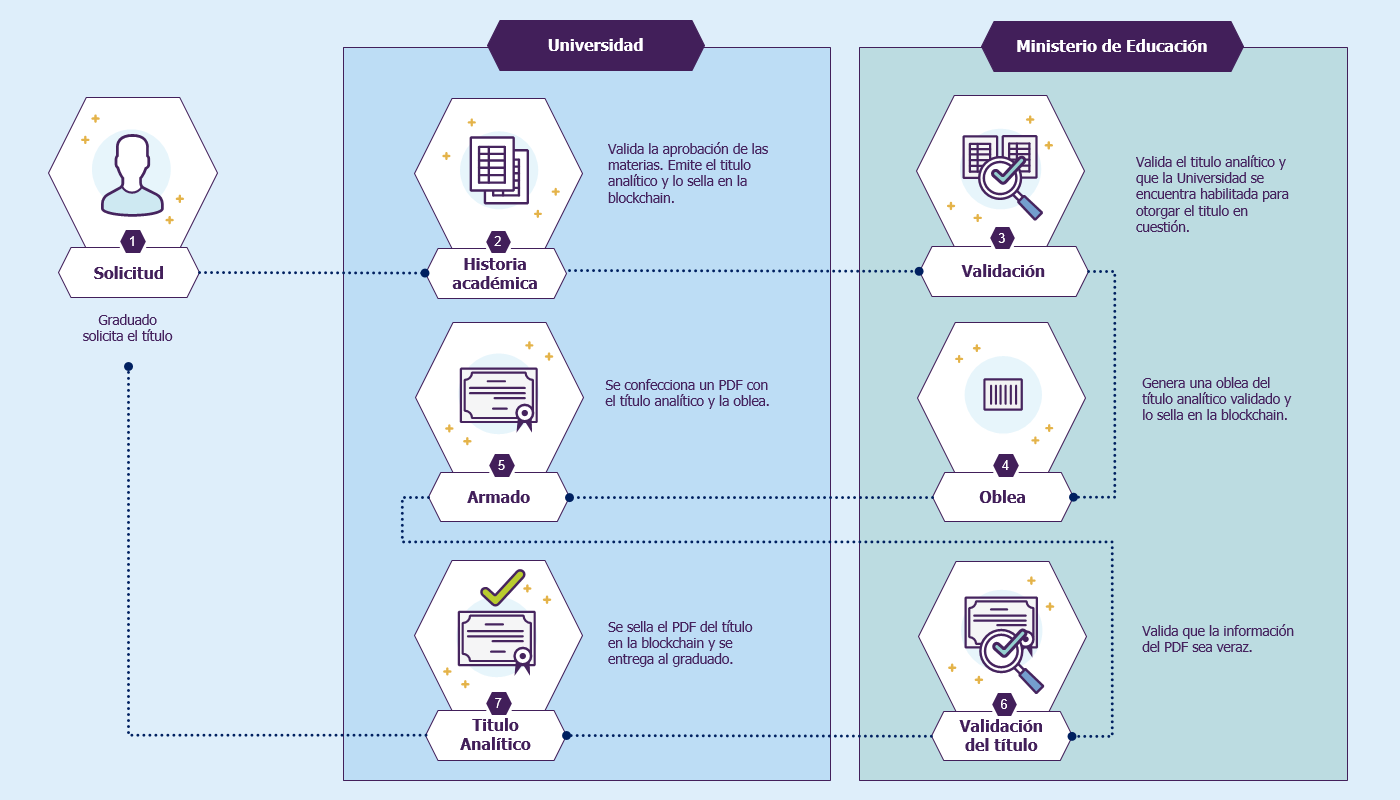
\includegraphics[width=\textwidth]{Img/cuadro_problematica.png}
            \caption{}
            \label{fig:cuadro_problematica}
        \end{figure}

        \subsection{Smart Degress}
        
        Smart Degress es una plataforma que permite al usuario mediante una Dapp la registracion y
        certificacion de diplomas y titulos academicos. Esto lo hace basandose en la premisa de que el 
        exito en el mercado laboral, depende de la certificacion de los titulos obtenidos.

        Para lograr su objetivo emplean la tecnologia blockchain con la cual proporcionan y añade una mayor agilidad,
        comodidad y seguridad. Con lo cual permite gestionar y compartir el titulo universitario en plataformas de trabajo, 
        reclutadores y terceros.


    \section{Objetivos}

    \section{Desafíos}

    \section{Etapas}

    \section{Conclusiones}

\end{document}